\documentclass[]{article}
\usepackage[]{graphicx}
\usepackage[]{xcolor}
\usepackage[]{minted}
\usepackage[utf8]{inputenc}

\begin{document}
\author{Matteo Ielacqua}
\title{Github Social}
\maketitle
    \section{Brief introduction}
    A large social network of GitHub developers which was collected from the public API in June 2019. Nodes are developers who have starred at least 10 repositories and edges are mutual follower relationships between them.
    \subsection{Context}
    GitHub is a double scope platform: In first place is used to store and develop software , either by open source developers and by companies, secondly is a social network for developers in which them can argue about technical solution and future projects. In GitHub a user can Fork ( copy the repository in his own userspace), view the code and star a repository. The star operation is a follow operation, thus a user can track the progress on certain repository. But is also possible to follow a developer to see which project he taken part to, and that's what the network is collecting. The original scope of this network was to target each developer (node) and understand if it is a machine learning or web developer, the content of this information is available in the file musae\_git\_target.
    
    \subsection{What to expect}
    This is a social network, so we expect a sparse graph with very few node very popular and most of them not. Most of the nodes should be part of a giant component. Triadic closure is probably given by some developers working on the same project (assumpting that the node is respecting the requirements of have starred 10 repositiories) and so we expect the presence of some big communities given by the presence of big project (like for example Unreal Engine source code or Qt company code). Sure there will a clearly manifestation of homophily, especially in those project oriented only in machine learning or webdesign, but what about bigger project that requires some exchanges of competences? The answer in obvliviously that heterophily has to be seen in those contexts. 

    \section{Basic Measures}
    
    \subsection*{Number of nodes and links}
    nodes in the network are : 37700, meanwhile links are : 289003. The dataset is indeed small, but large enough to allow some meaningful statistical measures. The network is connected, that means that there aren't disconnected subnetworks, so the largest connect component size is 37700.
    
    \subsection*{Density}
    Density is calculated using the formula $d=\frac{2L}{N(N-1)}$ where L is the number of links and N the number of nodes, this measure is taken by dividing the actual number of links on the maximum possible in this network. The result of this operation is 0.0004, such a low density is typical of social networks and this is one of them.

    \section*{Degree}   
    From a statistical view the subsequent data was obtained:
    \begin{itemize}
        \item Mean: 15.331724137931035
        \item Max: 9458
        \item Min: 1
        \item Variance: 6526.544335754138
    \end{itemize}
    The average degree is indicating that most of nodes have few connection to others, comparing this measure with the maximum and the variance it's reasonable to say that there are nodes very popular while there are others quite unknown, this behaviour is in line with the social networks ones. The average degree can be used to calculate the density with the following formula $$d=\frac{<k>}{N-1}$$ where $<k>$ is the average degree and N is the total number of nodes, again the result is 0.0004 confirming that both density and average degree are correct. 

    \subsection*{Degree distribution}

    \begin{center}
        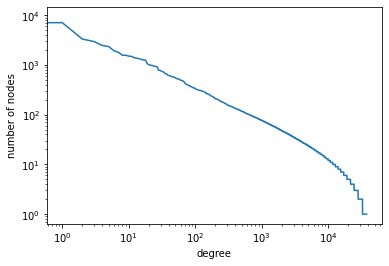
\includegraphics[scale=0.50]{charts/degree_dist_plot.png}
        \end{center}
    Plotting the histogram of degree distribution the following can be found:
    The chart clearly expose the difference in the degree distribution, mostly of the nodes are unknown but very few nodes are very popular, perhaps indicating that some power law can be present in the distribution of this measure. \\
    Using the module powerlaw from python the following chart of the cumulative distribution function (ccdf) is obtained:
    \begin{center}
    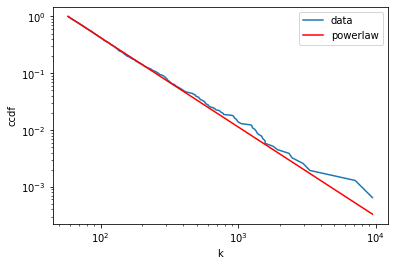
\includegraphics[scale=0.5]{charts/powerlaw.png}
    \end{center}
    In the chart the red line is the ccdf of a powerlaw, meanwhile the blue line is the ccdf of the degree. Comparing the line is visible that the degree distribution is following a power law of type $f(k) \propto k^{-\alpha}$, the module also can estimate $\alpha$ that assumed the value 2.5733, meaning that the degree distribution is not only a power law but is also in the scale free regime because the exponent is in the interval [2,3].


    

\end{document}